\documentclass[sigconfl]{acmart}

\usepackage{pdfpages}
\begin{document}

\title[Towards user-friendliness in theorem provers]{Towards user-friendliness
  in proof assistants: automated strategies \textbf{via} algebraic effects and handlers}

% \author{April Gonçalves}
% \email{april@metastate.dev}
% \affiliation{
%   \institution{Metastate}
%   \city{Edinburgh}
%   \state{UK}
% }

% \renewcommand{\shortauthors}{April Gonçalves}

\begin{abstract}
Proof assistants provide a framework for modelling and verification of
theories, as well as trust-worthy software. However, such power is usually only
available to experts. We propose a new approach, based on algebraic effects and
handlers, to integrate different automated proof strategies that enables
newcomers to take advantage of proof assistants without a more in-depth
understanding of underlying theory. Our approach gives beginner users an effect
system, a handful of effectful strategies (tactics, proof search and a SMT
solver) and their handlers under a shared interface, while advanced users can
extend our system with new effects and new handlers. Lastly, we prototype the
system as a library in Agda. While our prototype is minimal, it shows how easily
proofs can be carried on so long as the user has the correct intuition. We
believe our system empowers non-experts and has the potential to bring verified
software to many relevant industries, such as finance.
\end{abstract}

\keywords{effect handlers, proof assistants, user experience}

\maketitle

\section{Verification for the Masses}

The usability of proof assistants such as Coq, Agda, Isabelle/HOL and Twelf is
hard to measure: all of them require significant domain knowledge that
frequently matches a deeper understanding of Type Theory, the theory that
enables such assistants to exist. Coq and Isabelle/HOL are more commonly applied
outside their niche, and their programming style is sharply different from
mainstream programming and even functional programming. Granted, they come with
their own integrated development environment (IDE), which may make it easier for
students and newcomers. To our knowledge, no usability study has been
held for a proof assistant, however there exists studies that account for
an informal ``usability'' criteria -- they appear to measure how fast users can
familiarise themselves with the system or IDE.

Folklore within the proof assistants community seems to show that typical users
find Coq hard to use due to a large library of tactics and difficult readability
of the code after its completion. Many Coq learning materials suggest users to
add comments for structural induction cases and inductive hypothesis. As
mentioned, no user studies were conducted to attest such hypotheses.

It also has to be granted that proof assistants are relatively new technology
and there are no guidelines or even an intuition on how such systems should
perform or what features should be available to the users. The closest model we
have are proofs by hand, however, following that model for proof assistants has
two main pitfalls: (a) proofs by hand are also not widely taught in mathematics
classes during school years; and (b) proofs by hand and automated proof
writing employ fundamentally different paradigms, where the latter requires
axioms and formulations to be encoded explicitly, commonly known as a ``pedantic
proof style''.

\subsection{Empowering users of different levels of expertise}

To popularise software verification, we mush make proof writing less of a
burden to the user. Currently, only specialists can write proofs for their
programs, even though the working programmer understands the domain and
invariants of their projects -- otherwise they would not be able to write any
software. \textit{Our hypothesis is that programmers are well-equipped to derive and
prove properties of the software they write, but they lack the mathematical maturity and
vocabulary to carry out a formal proof. } We have evidence that students fail to
produce well-made proofs due to the lack of mathematical maturity, even though
they do understand the subject matter at hand.

In our approach, we propose an (algebraic) effects and handlers view of such
proofs, based on prior work developed by the Andromeda proof assistant. Here,
our users will program as they would normally and invoke
a proof environment as an effect to prove certain properties as they go. Given
that the proof environment is \textit{just} an effect, we envision that different proof
styles (e.g, Agda-style dependent types, SMT solver, proof search) can be ``composed''
under a shared interface, a proof object that can manipulate itself while
enquiring different automated proof engines.

The reasons we employ algebraic effects and handlers are manifold:
\begin{enumerate}
\item as proofs cannot be fully automated, all approaches that try to automate
  the process (e.g, proof search, SMT solver) may either be non-deterministic or
  never find a solution. Therefore, the system should be able to handle
  ``impure'' computations and errors. Algebraic effects and handlers have
  well-defined semantics and provide a simple interface for performing effects.
  With them, we avoid indiscriminate effects that are often error-prone and
  intricate effects machinery such as monad transformers;
\item its semantics accommodate composition of arbitrary effects and the
  composition of multiple handlers, which means users have the ability to weaken
  more general strategies into specific ones while maintaining the original untouched;
\item it has well-defined semantics, and it is the main feature of many new
  research languages, such as Koka, Eff, Frank and Effekt, what suggests a greater
  potential.
\end{enumerate}

\subsection{Goals and Contributions}

The present project intends to land itself as a compiler-level implementation into the
Juvix\footnote{Juvix is a dependently-typed programming language for smart
  contracts. More information at juvix.org} programming language. We design
Juvix with focus on working programmers familiar with strongly-typed functional
programming.

\paragraph{Goals} The project exists to enable users to write safe, verified
code without investing time into learning dependent types and theorem proving.
The project's goals are presented as follows:
\begin{enumerate}
\item make software verification more accessible to programmers familiar with
  functional programming;
\item foster knowledge sharing between domain experts and regular programmers;
\item lower the barrier to entrance into software verification to non-experts.
\end{enumerate}

\paragraph{Contributions} While the project is a work-in-progress, this paper
provides three important contributions that lays out the full extent of the
work, which are presented as follows:
\begin{enumerate}
\item a specification of a user interface for automated proofs based on
  algebraic effects and handlers that permits user-defined effects for proof
  strategies, and also user-defined handlers for existing effects (Section \ref{intro-witch});
\item a minimal prototype in Agda that validates the feasibility of such system
  (Section \ref{witch-agda});
\item a short technical account of the effort required to materialise such a
  user interface into proof assistants (Section \ref{tech-details}).
\end{enumerate}

\section{Introducing Witch} \label{intro-witch}

\begin{figure}[!ht]
   \centering
    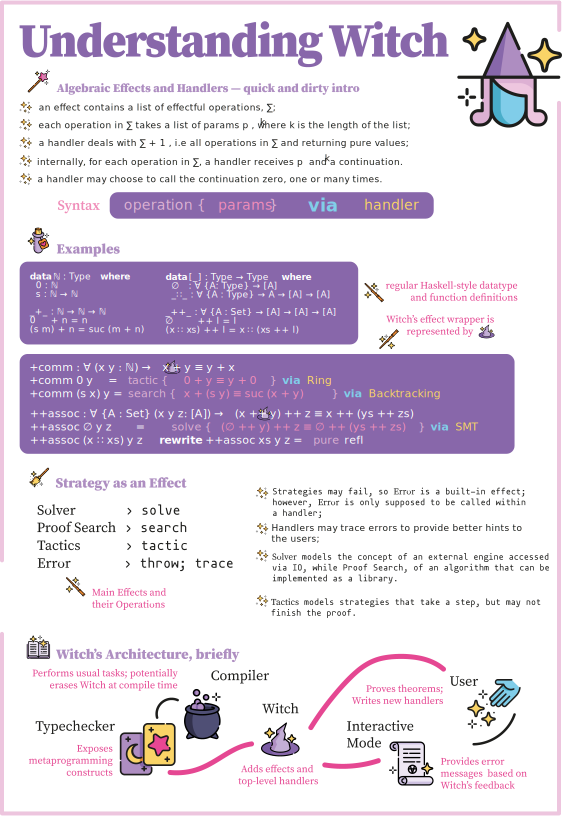
\includegraphics[height=\textheight]{image/witch.eps}
    \caption{Summary of Witch pertaining to strategies, examples
      and the architecture.}
    \label{fig:prototype}
\end{figure}

In this section, we introduce our approach, named Witch\footnote{Our tool's name is
  a play after assistant tools colloquially called ``wizards''. There is no
  consensus of what a wizard is or what are exactly the tasks it is supposed
  to help users. Wizards seem to be used mostly for multiple-step and/or
  configuration features, however. We went for the name ``witch'' to align it to
the idea of assistant tools, while dodging the overloaded, yet nebulous
terminology.}. We define a \textit{witch} as an assistant tool for theorem
provers that congregates many different strategies for proof automation. Our
specification for a \textit{witch} for Juvix uses algebraic effects and handlers
as the means to congregate strategies as effects.

\paragraph{Algebraic Effects and Handlers} Algebraic effects were introduced by
**citation, and their handlers were introduced later on by **citation. An
algebraic effect is defined by an effect signature that comprises a set of
operations, and handlers that denote said operations. A handler may interpret
operations at the compiler-level, which was formally named co-model, but
colloquially called ``top-level handler''. Handlers are the most general form to
denote a set of operation, and more specific classes of handlers also exist.

\paragraph{The Essence of Witch}
In Figure \ref{fig:prototype}, we sum up our \textit{witch} approach.
As for the syntax, we use \texttt{operation \{ params \} via handler} that is an
improvement over \texttt{handler(operation, params)}, since effect handling is similar
to function application where it carries effect information as well.
The user defines data types and functions as usual, and then uses a
\textit{witch} to prove properties concerning said definitions. The Examples
section in Figure \ref{fig:prototype} shows it in action. The examples are
over-simplified to enable a clearer communication of our proposal -- we avoid
more complex properties and complicated proofs as initial examples. The proof of
commutativity of addition under natural numbers and of associativity of list
concatenation are shown, and use the three main effects: Solver, Proof Search
and Tactics. In the proof assistant literature, there exists no precise
definition of commonly used terms ``solver'', ``proof search'' and ``tactics''.
All said terms are used in different communities to mean ``automatic strategy to
construct a term under certain constraints''. Here, however, we opt for a
pragmatic differentiation:
\begin{itemize}
  \item The Solver effect is used for integration with external engines via IO;
    we believe it suffices to say, e.g. \texttt{SMT}, as handlers should
    implement internal strategies to choose between the so-called logics
    within a solver. If the black-box approach to solvers presents itself a
    challenge, an specialisation of the handler is possible, e.g.
    \texttt{operation \{ params \} via Z3.QF-UFLIA}.
  \item The Proof Search effect is used for library-level algorithms; users may
    choose to implement their own algorithms using a limited set of
    meta-programming constructs that are handled at top-level\footnote{The
      meta-programming constructs are operations of the Typechecker effect
      whose handlers are not available for the user.}.
    \item The Tactics effect represent strategies that simplifies the proof at
      least one step, and may not complete all proof goals. This style is mainly
      employed in the proof assistant Coq. While we do not foresee as many
      tactics implemented as in Coq, we believe famous tactics such as
      \texttt{omega}, \texttt{ring}, \texttt{Admitted} are useful to users of
      all levels of expertise.
    \item Lastly, the Error effect represents feedback messages to the user,
      since any of the strategies may fail. Error has two operations,
      \texttt{throw} and \texttt{trace}: the former notifies the user a strategy
      has failed, while the latter registers\footnote{Internally, the
        Typechecker effect should have a tree that stores all currently
        saved traces.} completed sub-goals during the
      strategy's attempt to complete the proof.
\end{itemize}

\paragraph{Witch's Architecture}
A \textit{witch} sits between the typechecker and the interactive mode of a
proof assistant. It uses constructs provided by the typechecker and notifies the
interactive mode with regards to the state of the current strategy attempted.
The user may manipulate proof handlers by composing or writing their own.



\paragraph{Downsides of our Approach}
There are two main styles for writing proofs within a proof assistant: external
verification and internal verification. The latter concerns itself with code
that is \textit{correct-by-construction}, meaning that only valid states can be encoded and it
carries all information necessary to make proofs trivial; while the former
concerns itself with proofs about code that does not carry any additional
information for proving purposes.
Witch's primarily focus is on external verification. We believe that newcomers
will struggle to write proof-aware code, since it departs strongly from
mainstream programming, even within the functional style. We expect users to
write their code as they normally would do and then prove necessary properties.
Witch does not support writing correct-by-construction code. As proofs
are erased during compilation-time in Juvix, Witch could be extended
to be indexed by proof objects and parameterised over any type, such as
\texttt{\{A: Type\} $\rightarrow$ x y: A $\rightarrow$ }
\includegraphics[height=0.02\textheight]{image/hat.eps} \texttt{ (x * y $\equiv$
  y * x) } where we make sure that \texttt{*} over \texttt{A} is commutative.
However, it is unclear whether having user's code under a monad-like structure leads
to well-structured code.

\section{Agda's Witch} \label{witch-agda}





\paragraph{Why Agda?} Agda provides higher-level meta-programming constructs, and
its coding style is a reminiscent of the ML family of functional programming languages.

\subsection{Technical Effort Required} \label{tech-details}

Although Witch is implementable at the library level, it requires that proof
assistants to provide a set of off-the-shelf features. The most important
feature is type-level meta-programming. Witch is only possible given the proof
assistant's ability to manipulate its own proof terms to generate new variables,
holes, goals, among others and manipulate terms and types in a proof-carrying
fashion. Secondly, the proof assistant should feature an interface with the
outside world. Although it is not inherently a requirement, its absence means
that no solver will be integrated, diminishing the proposed value of the tool.
Lastly, proof assistants must support algebraic effects and handlers. If there
is no built-in solution, a library-level solution is possible -- as we did in
Agda. However, a solid implementation may not be trivial to achieve. In Agda,
we translate effect handling into optimised continuation-passing style that inlines
all applications. This strategy also works at compiler-level if necessary. There exist
many strategies to efficiently implement algebraic effects and handlers, but we
went for the one that seemed the most straight-forward method to implement it in Agda.

\section{Related and Future Work}

While it is hard to say whether we have achieve our goals before user
evaluations, Witch steps towards a future where proof assistants are
friendlier towards users, particularly newcomers. The present work is in its
infancy, and there are many issues concerning Witch's ability to guide newcomers
towards correct-by-construction software, which constitutes the main improvement
we intend for Witch. We hypothesise about the possibility of using proof
reconstruction, therefore relocating Witch to an assistant that lives solely
within the interactive mode -- as opposed to a framework for proof
automation in user code.

In parallel with the usability work, we plan to develop a formalisation of Witch
as a dependent typed language with effectful, dependently typed operations and
effect handler, based on previous work on fibred algebraic effects.

\end{document}
\endinput
